% 无封面页
\documentclass[withoutpreface]{cumcmthesis}

\begin{document}

\begin{abstractpage}{常见的一维插值方法汇总}
    本文主要研究常见的一维插值方法。

    首先,我们阐述了一维插值的定义与作用。
    其次,我们证明了以$n+1$个插值节点获得$n$次插值多项式的存在性与唯一性,并引入了\textbf{待定系数法}、\textbf{拉格朗日插值法}、\textbf{牛顿插值法}这三种单一多项式函数插值方法。
    然后,我们展示了单一多项式函数插值方法随着$n$增大可能出现的\textbf{龙格震荡现象},并介绍了为了解决这个问题常用的两种分段多项式函数插值方法———\textbf{分段线性插值}和\textbf{三次样条插值},给出了相应的示例图。
    最后,我们总结全文,推荐在日常应用中,使用分段线性插值和三次样条插值。
    \keywords{插值 \quad 龙格现象 \quad 多项式插值 \quad 分段插值 \quad 样条插值}
\end{abstractpage}

\tocpage
\section{一维插值问题简介}

已知函数$y=f(x)$上的$n+1$个数据点$(x_0,y_0),(x_1,y_1),(x_2,y_2),\cdots,(x_n,y_n)$,而函数的表达式未知,要求从某类函数(如多项式函数、样条函数等)中求得一个函数$\varphi(x)$,使得$\varphi(x)$通过这已知的$n+1$个点,即$f(x_i)=\varphi(x_i),i=0,1,2,\cdots,n$。求得$\varphi(x)$后,便可以通过$\varphi(x)$在其他观测点上的函数值来近似$f(x)$的函数值。这样的数学问题就称为\textbf{一维插值问题}。

在数学建模分析过程中,数据常常缺少或者不足以支撑分析的进行,这种时候,就需要使用插值方法来“模拟产生”一些新的但具有一定合理性的数据。

常见的一维插值方法是利用多项式函数来进行插值。

\section{单一多项式函数插值}
\subsection{待定系数法确定插值多项式}

设插值函数为一个$n$次多项式,即
\begin{equation}\label{1}
    \varphi(x)=a_0+a_1x+a_2x^2+\cdots+x^n
\end{equation}

将$n+1$个已知数据点代入,得到一个关于$a_0,a_1,\cdots,a_n$的$n+1$元一次方程:
\begin{equation}\label{2}
    \begin{cases}
        \varphi(x_0) = a_0+a_1x_0+a_2x_0^2+\cdots+a_nx_0^n = f(x_0) \\
        \varphi(x_1) = a_0+a_1x_1+a_2x_1^2+\cdots+a_nx_1^n = f(x_1) \\
        \cdots                                                      \\
        \varphi(x_n) = a_0+a_1x_n+a_2x_n^2+\cdots+a_nx_n^n = f(x_n) \\
    \end{cases}
\end{equation}

\cref{2}的系数行列式为
\begin{equation}
    d=
    \begin{bmatrix}
        1      & x_0    & x_0^2  & \cdots & x_0^n  \\
        1      & x_1    & x_1^2  & \cdots & x_1^n  \\
        \cdots & \cdots & \cdots & \ddots & \vdots \\
        1      & x_n    & x_n^2  & \cdots & x_n^n  \\
    \end{bmatrix}
\end{equation}

d 是一个典型的范德蒙德 (Vandermonde) 行列式,又$x_0\ne x_1 \cdots \ne x_n$,则$d\ne 0$。由克莱姆法则得,系数行列式不为0的方程组有且仅有一个非零解。所以可以得出一个结论,\textbf{插值多项式函数$\varphi(x)$有且仅有一个}。

然而,直接通过解\cref{2}来求插值多项式函数$\varphi(x)$是不现实的。主要原因就是,当$n$较大时,方程组变得难以使用计算机求解或需要花费较多资源来求解。

下文会提到构造插值多项式函数的拉格朗日插值法和牛顿插值法,它们用计算机实现起来比较简单,不过求得的插值多项式函数其实都是相同的。

\subsection{拉格朗日插值法}

多项式插值函数是一定存在且唯一存在的,但通过求方程组的解难以求得。

拉格朗日插值法是一种寻找多项式插值函数的简便方法。

首先,构造一组\textbf{基函数}
\begin{equation}
    l_i(x) = \frac{(x-x_0)\cdots(x-x_{i-1})(x-x_{i+1})}{(x_i-x_0)\cdots(x_i-x_{i-1})(x_i-x_{i+1})}
    =\underset{j=0}{\prod \limits_{j\ne i}^n}\ \frac{x-x_j}{x_i-x_j}
\end{equation}

易知$l_i(x_j)=\begin{cases}
        0 & j\ne i \\
        1 & j=i
    \end{cases}$

进而构造
\begin{equation}
    L_n(x) = \sum\limits_{k=0}^{n} l_k(x)f(x_k)
\end{equation}

则
\begin{equation*}
    L_n(x_i) = \sum\limits_{k=0}^{n} l_k(x_i)f(x_k)=l_i(x_i)f(x_i) = f(x_i)
\end{equation*}

即$Ln(x)$满足插值函数的条件。又多项式插值函数唯一,则$L_n(x)$就是\cref{1}

\subsection{牛顿插值法}

牛顿插值法也是一种寻找多项式插值函数的简便方法。它使用到了所谓\textbf{差商}的概念。

\begin{definition}[差商]
    设有函数$f(x),x_0,x_1,x_2,\cdots$为一系列互不相等的观测点。

    称\begin{equation*}
        \frac{f(x_i)-f(x_j)}{x_i-x_j}
    \end{equation*}为$f(x)$关于点$x_i,x_j$的一阶差商,简称差商,记为$f[x_i,x_j]$

    称一阶差商的差商\begin{equation*}
        \frac{f[x_i,x_j]-f[x_j,x_k]}{x_i-x_k}
    \end{equation*}为$f(x)$关于点$x_i,x_j,x_k$的二阶差商,记为$f[x_i,x_j,x_k]$

    一般地,称
    \begin{equation*}
        \frac{f[x_0,x_1,\cdots,x_{n-1}]-f[x_1,x_2,\cdots,x_n]}{x_0-x_n}
    \end{equation*}
    为$f(x)$关于$x_0,x_1,\cdots,x_n$的$n$阶差商,记为$f[x_0,x_1,\cdots,x_n]$。
\end{definition}

根据差商的定义,我们有
\begin{align*}
    f(x)=                        & f(x_0)+(x-x_0)f[x,x_0]                                       \\
    f[x,x_0]=                    & f[x_0,x_1]+(x-x_1)f[x,x_0,x_1]                               \\
    f[x,x_0,x_1]=                & f[x_0,x_1,x_2]+(x-x_2)f[x,x_0,x_1,x_2]                       \\
    \cdots                                                                                      \\
    f[x,x_0,x_1,\cdots,x_{n-1}]= & f[x_0,x_1,x_2,\cdots,x_n]+(x-x_n)f[x,x_0,x_1,x_2,\cdots,x_n]
\end{align*}

上式依次乘$1,(x-x_0),(x-x_0)(x-x_1),\cdots,(x-x_0)(x-x_1)\cdots(x-x_{n-1})$再相加,得到
\begin{equation*}
    f(x)=f(x_0)+(x-x_0)f[x_0,x_1]+(x-x_0)(x-x_1)f[x_0,x_1,x_2]+\cdots
\end{equation*}
\begin{equation*}
    +(x-x_0)(x-x_1)\cdots(x-x_{n-1})f[x_0,x_1,\cdots,x_{n-1}]
\end{equation*}
\begin{equation*}
    +(x-x_0)(x-x_1)\cdots(x-x_{n})f[x,x_0,x_1,\cdots,x_{n}]
\end{equation*}


记基函数为$N_i(x)=f[x_0,\cdots,x_{i}] \prod \limits_{k=0}^i(x-x_k)$,则
\begin{equation}
    f(x)=f(x_0)+\sum\limits_{i=0}^{n-1}N_i(x)+(x-x_0)(x-x_1)\cdots(x-x_{n})f[x,x_0,x_1,\cdots,x_{n}]
\end{equation}

记$N(x)=f(x_0)+\sum\limits_{i=0}^{n-1}N_i(x)$,则$N(x)$满足插值条件,且最高次数为$n$,由多项式插值函数的唯一性得,$N(x)=\varphi(x)$

\subsection{龙格震荡现象}

使用单一多项式函数进行插值,随着$n$的增大,可能会出现插值函数震动幅度太大,即所谓\textbf{龙格震荡现象},导致插值效果不太理想。

例如,考虑$f(x)=\frac{1}{x^2}$,以其$n+1$个节点插出$n$次多项式函数$\varphi_n(x)$,取$n=6,8,10$

\begin{figure}[H]
    \centering
    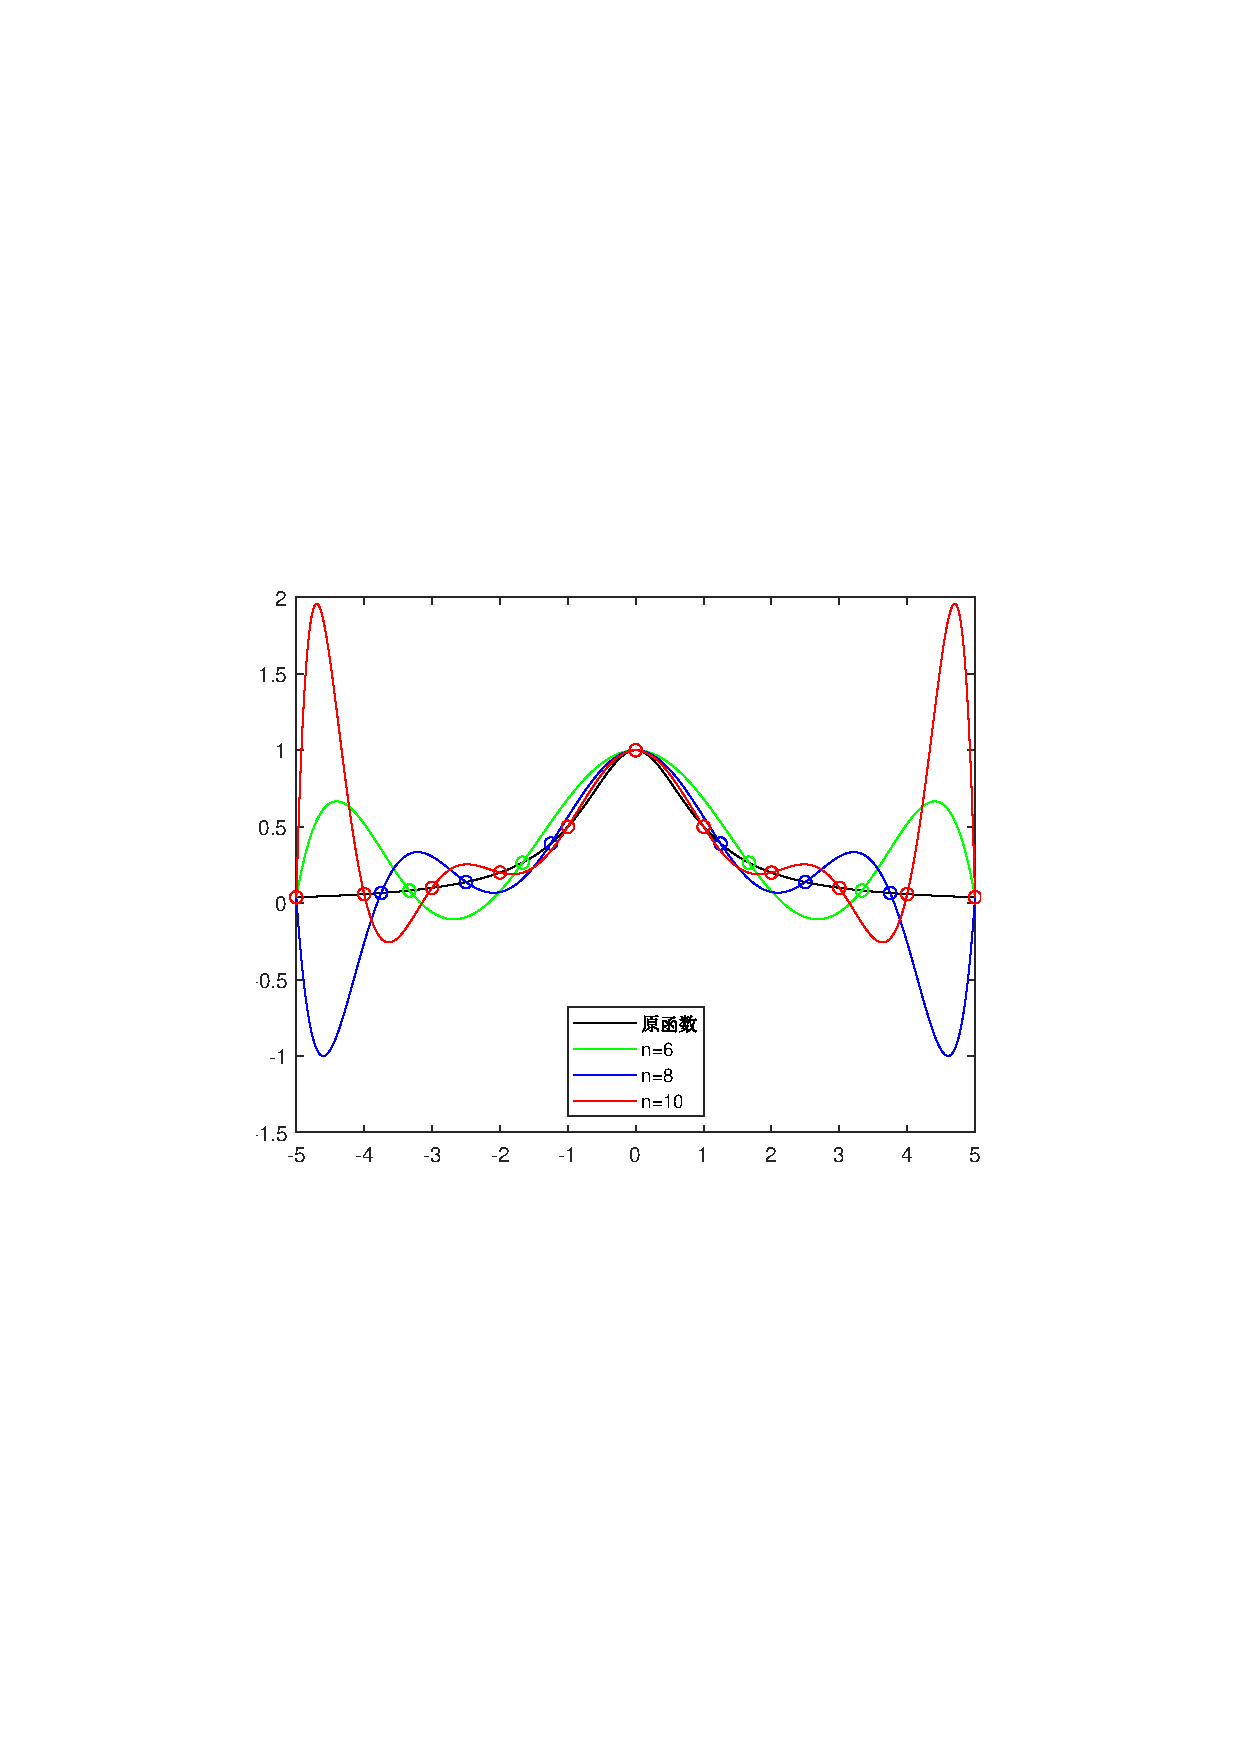
\includegraphics[width=0.5\textwidth]{龙格现象}
    \caption{龙格震荡现象示例}
\end{figure}

\section{分段多项式函数插值}

单一多项式插值往往因为插值函数次数太高而出现龙格震荡现象导致插值效果不好,为了解决这个问题,可以使用\textbf{分段多项式函数}来进行插值。各段多项式次数都很低,一般能取得较好的插值效果。

\subsection{分段线性插值}

最简单的分段多项式插值当然是\textbf{分段线性插值},即线性连接相邻的插值节点整体形成一个插值函数。

分段线性插值的好处是,它不仅能避免龙格震荡现象,而且当插值节点越多的时候,最后得到的插值函数与原函数越接近,即$\lim \limits_{n \to \infty} \varphi_n(x) = f(x)$

\begin{figure}[H]
    \centering
    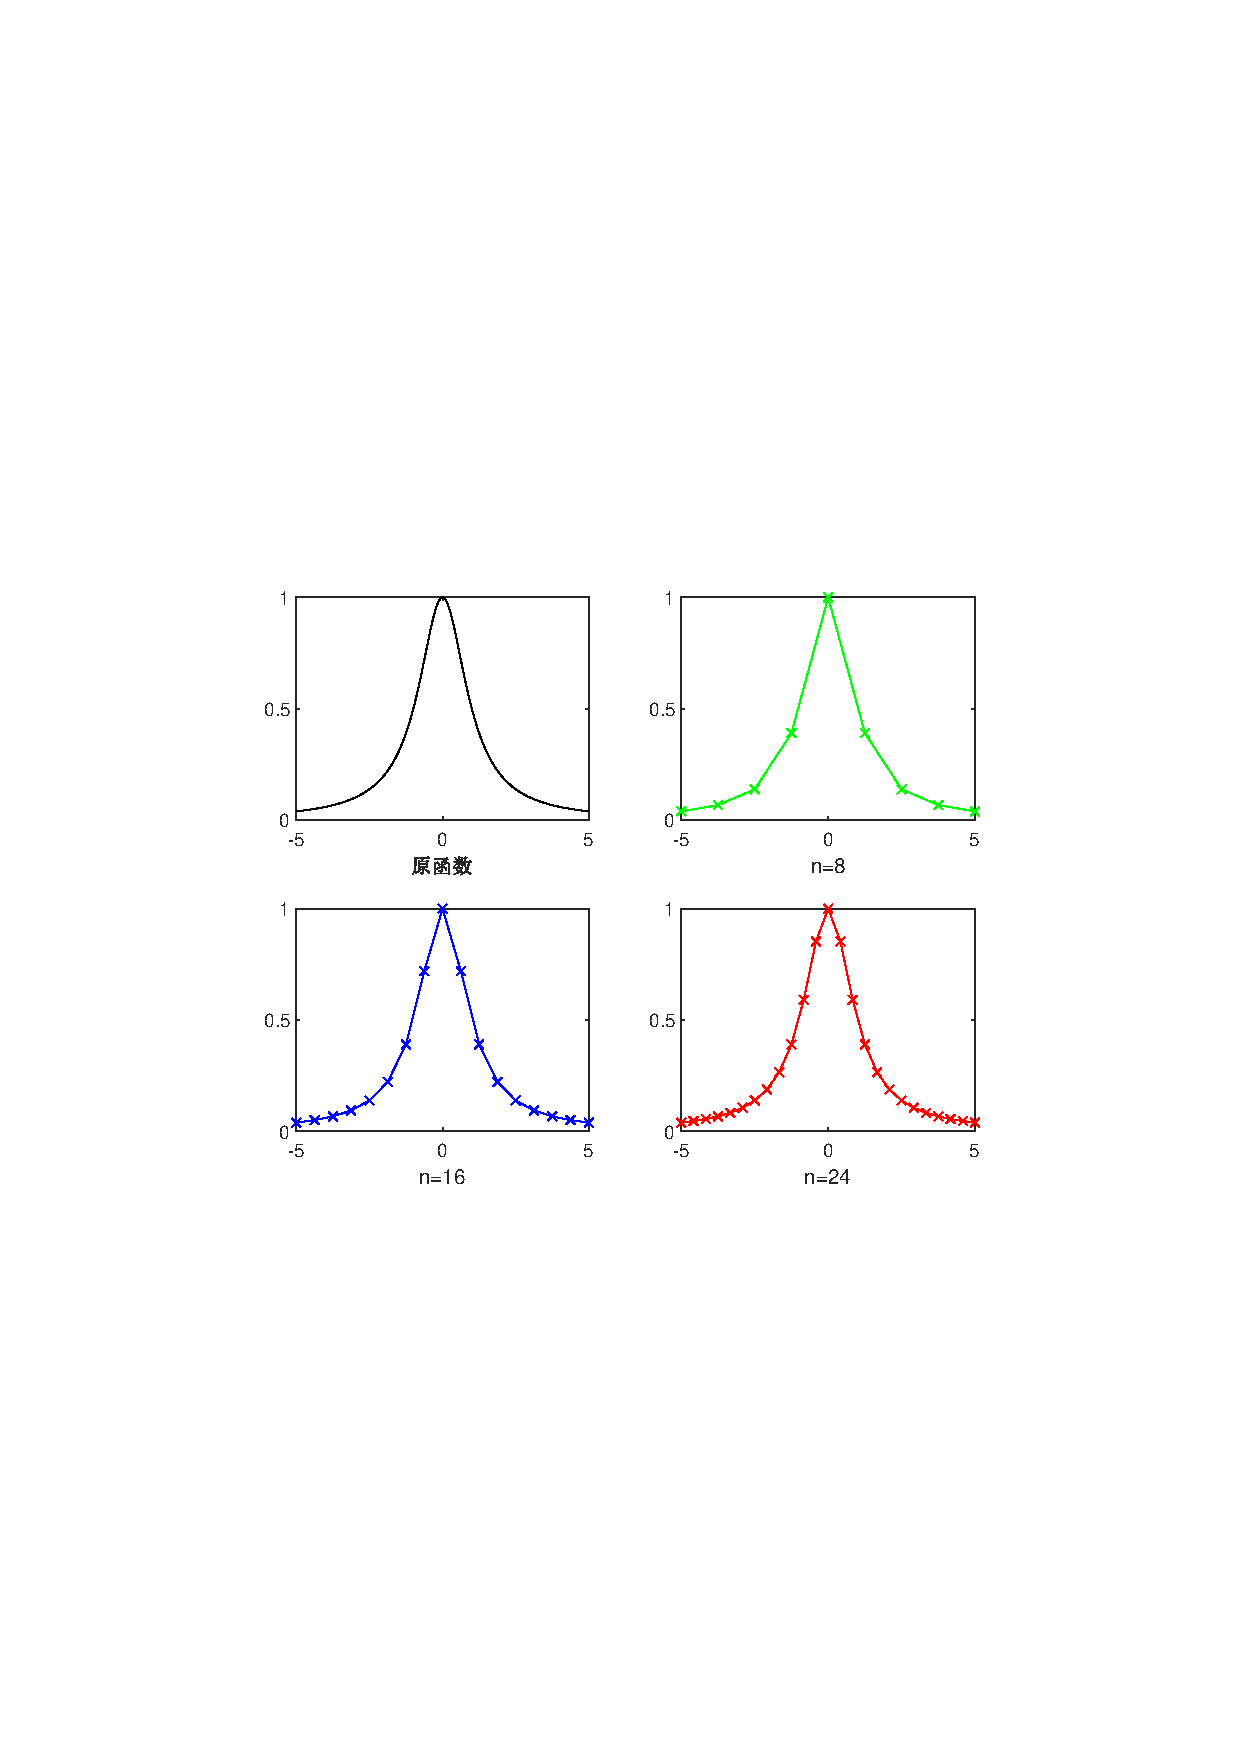
\includegraphics[width=0.8\textwidth]{分段线性插值}
    \caption{分段线性插值示例}
\end{figure}

一般的应用场景下,使用分段线性插值就已经足够了。

\subsection{三次样条插值}

分段线性插值有一个很明显的缺点:它不够光滑。尤其是在插值节点处,分段线性插值函数甚至不存在一阶导数。要解决这个问题,我们可以采用\textbf{样条函数}进行插值。

\begin{definition}[样条函数]
    样条函数实际上也是一种分段多项式函数。如果定义在$[a,b]$上的函数$S(x)$满足:
    \begin{enumerate}
        \item 给定$[a,b]$的一个分划$\Delta:a=x_0<x_1<\cdots<x_n=b$,在每个小区间$[x_i,x_{i+1}]$上,$S(x)$都是$k$次多项式函数。
        \item $S(x)$在$[a,b]$上具有$k-1$阶连续导数
    \end{enumerate}
    则称$S(x)$是关于分划$\Delta$的$k$次样条函数。$k$次样条函数$k-1$次光滑。
\end{definition}

\vspace{-0.4cm}
最常见的做法是使用\textbf{三次样条函数}来进行插值,它能保证插值函数在插值节点处存在二阶导数。

已知插值节点$(x_0,y_0),(x_1,y_1),\cdots,(x_n,y_n)$,对应的三次样条函数为$S(x)$。设$S(x)$在区间$[x_i,x_{i+1}],i=0,1,\cdots,n-1$上为$S_i(x)$,则$S(x)$必须满足以下条件:

\begin{itemize}
    \item \textbf{插值条件}\quad $S(x_i)=y_i,i=0,1,\cdots,n$
    \item \textbf{连续条件}\quad $S_i(x_{i+1})=S_{i+1}(x_{i+1}) i=0,1,\cdots,n-2$
    \item \textbf{一阶导连续}\quad $S'_i(x_{i+1})=S'_{i+1}(x_{i+1}) i=0,1,\cdots,n-2$
    \item \textbf{二阶导连续}\quad $S''_i(x_{i+1})=S''_{i+1}(x_{i+1}) i=0,1,\cdots,n-2$
\end{itemize}

$S(x)$在$n$个小区间上都是三次函数,有4个参数,因此求出三次样条函数需要确定$4n$个参数。而上面却只给出了$(n+1)+3(n-1)=4n-2$个条件。理论上还需要2个条件。我们可以根据实际情况自行补充。常见的有:
\begin{itemize}
    \item \textbf{自由边界条件}\quad $S''(x_0)=f''(x_0),S''(x_n)=f''(x_n)$
    \item   \textbf{固定边界条件}\quad $S'(x_0)=f'(x_0),S'(x_n)=f'(x_n)$
    \item \textbf{周期边界条件}\quad $S'(x_0)=S'(x_n),S''(x_0)=S''(x_n)$
\end{itemize}

求解三次样条函数的过程就不在此详解。可以参考数值计算相关书籍。

\begin{figure}[H]
    \centering
    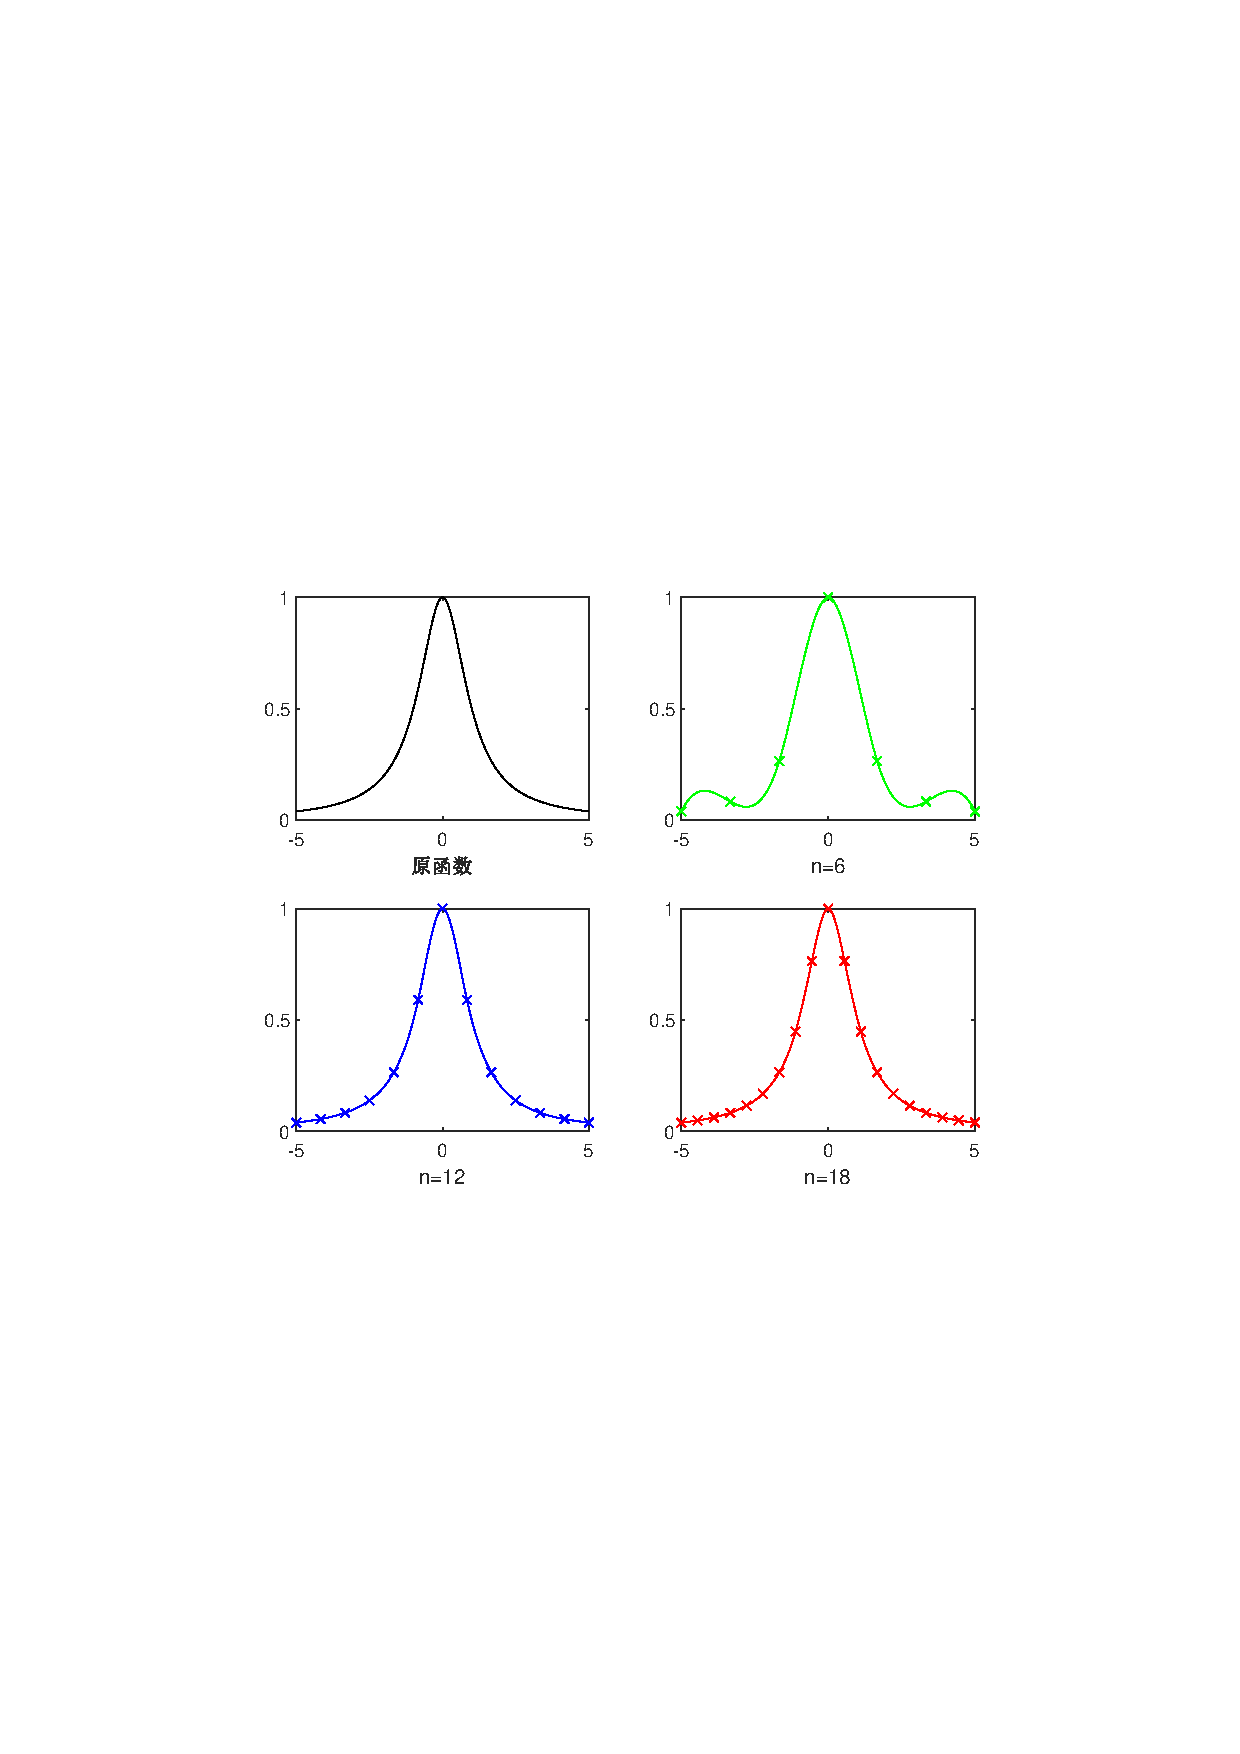
\includegraphics[width=0.63\textwidth]{三次样条插值}
    \vspace{-0.3cm}
    \caption{三次样条插值示例}
\end{figure}

\section{一维插值问题总结}

如果并不知道原函数的大体性质,那么没有一种插值算法可以说是最好的。不过,在实际运用中,为了避免龙格现象的出现,即插值的不稳定性,我们常常使用\textbf{分段线性插值}和\textbf{三次样条插值}。分段线性插值操作和性质都比较简单,而且插值节点越多效果越好;三次样条插值生成的曲线比较光滑,任意一点存在连续的二阶导数。

\appendix

\section{Matlab代码}

\begin{lstlisting}[language=matlab ,caption={待定系数方程组法} ]
    function y = SolveInterpolate(x0,y0,x)
    % 使用方程组法得到单多项式插值函数
    % x0,y0:已知的原始数据点
    % x,y:插值得到的点
    % x,y,x0,y0均为列向量
    
        %% 输入参数解方程 X a = y0 
        d = vander(x0);
        a = d \ y0;
        y = polyval(a,x);
    end
    \end{lstlisting}

\begin{lstlisting}[language=matlab ,caption={拉格朗日插值法} ]
    function y = LagrangeInterpolate(x0,y0,x)
        % 使用拉格朗日插值法得到单多项式插值函数
        % x0,y0:已知的原始数据点
        % x,y:插值得到的点
        
        %% 拉格朗日插值
        n = length(x0);
        m = length(x);
        y = ones(m,1);
        for k = 1:m
            x_new = x(k);
            y_new = 0;
            % 构造第i个基函数l_i,并代入第k个新x值,对l_i进行累加得到y_new
            for i = 1:n
                l_i=1;
                for j = 1:n
                    if j~=i
                        l_i = l_i * (x_new-x0(j))/(x0(i)-x0(j));
                    end
                end
                y_new = y_new + y0(i)*l_i;
            end
            y(k) = y_new;
        end
    end
    \end{lstlisting}

\begin{lstlisting}[language=matlab ,caption={求差商表} ]
    function dqTable = DifferQuotient(x,y)
    % 根据输入的x,y(n+1维)计算n阶差商
    
        n = length(x)-1;
        dqTable = cell(n+1,1);
        dqTable{1} = y;
        for j = 1:n
            delta_y = diff(dqTable{j});
            for i = 1:n-j+1
                delta_x = x(i+j)-x(i);
            end
            dqTable{j+1} = delta_y ./ delta_x;
        end
        dqTable = dqTable(2:end,:);
    end
    \end{lstlisting}

\begin{lstlisting}[language=matlab ,caption={牛顿插值} ]
    function y = NewtonInterpolate(x0,y0,x)
    % 使用牛顿插值法得到单多项式插值函数
    % x0,y0:已知的原始数据点
    % x,y:插值得到的点
    
        %% 牛顿插值
        n = length(x0);
        m = length(x);
        y = ones(m,1);
        
        % 计算差商
        dqTable = DifferQuotient(x0,y0);
        % 求第i个基函数并代入第k个新x值,结果相加
        for k=1:m
            x_new = x(k);
            Product = 1;
            N = y0(1);
            for i=1:n-1
                Product = Product*(x_new-x0(i));
                N = N + dqTable{i}(1,1)*Product;
            end
            y(k,1) = N;
        end
    end
    \end{lstlisting}

\begin{lstlisting}[language=matlab ,caption={插值问题主体} ]
    clear,clc
    %% 定义原函数
    f = @(x) 1./(1+x.^2); 
    %% 绘制原函数
    x = -5:0.01:5;
    y = f(x);
    plot(x,y,'black');
    hold on;
    %% 绘制单段多项式插值函数
    color = ["green","blue","red"];
    for n = [6,8,10]
        x0 = linspace(-5,5,n+1);
        y0 = f(x0);
        new_y = NewtonInterpolate(x0,y0,x);
        plot(x0,y0,color(n/2-2)+'o',x,new_y,color(n/2-2));
        hold on
    end
    legend("原函数","","n=6","","n=8","","n=10","Location","south");


    clc,clear
    %% 定义原函数
    f = @(x) 1./(1+x.^2); 
    %% 绘制原函数
    x = -5:0.01:5;
    y = f(x);
    subplot(221)
    plot(x,y,'black');
    xlabel("原函数")
    %% 绘制线性插值函数
    color = ["green","blue","red"];
    for n = [8,16,24]
        x0 = linspace(-5,5,n+1);
        y0 = f(x0);
        new_y = interp1(x0,y0,x,"linear");
        subplot(221+n/8);
        plot(x0,y0,color(n/8)+'x',x,new_y,color(n/8));
        xlabel("n="+n);
    end
        
        
    clc,clear
    %% 定义原函数
    f = @(x) 1./(1+x.^2); 
    %% 绘制原函数
    x = -5:0.01:5;
    y = f(x);
    subplot(221)
    plot(x,y,'black');
    xlabel("原函数")
    %% 绘制三次样条插值函数
    color = ["green","blue","red"];
    for n = [6,12,18]
        x0 = linspace(-5,5,n+1);
        y0 = f(x0);
        new_y = interp1(x0,y0,x,"spline");
        subplot(221+n/6);
        plot(x0,y0,color(n/6)+'x',x,new_y,color(n/6));
        xlabel("n="+n);
    end
    \end{lstlisting}

\section{Python 代码}

    \begin{lstlisting}[language=python ,caption={初始化} ]
    import numpy as np
    import matplotlib.pyplot as plt
    from scipy import interpolate
    
    np.set_printoptions(suppress=True)
    
    plt.rcParams["font.sans-serif"] = ["SimHei"]  #设置字体
    plt.rcParams["axes.unicode_minus"] = False  # 解决图像中的“-”负号的乱码问题
    \end{lstlisting}

    \begin{lstlisting}[language=python ,caption={待定系数方程法} ]
    def solve_interpolate(x0, y0, x):
    """使用方程组法得到单段多项式插值函数"""
        # 输入参数解方程 X a = y0
        d = np.vander(x0)
        a = np.dot(np.linalg.inv(d), y0)
        y = np.polyval(a, x)
        return y
    \end{lstlisting}

    \begin{lstlisting}[language=python ,caption={拉格朗日插值法} ]
    def langrange_interpolate(x0, y0, x):
    """使用拉格朗日插值法得到单多项式插值函数"""
    
        # 参数初始化
        n = len(x0)
        m = len(x)
        y = np.ones(m)
    
        for k in range(m):
            x_new = x[k]
            y_new = 0
            # 构造第i个基函数l_i,并代入第k个新x值,对l_i进行累加得到y_new
            for i in range(n):
                l_i = 1
                for j in range(n):
                    if j != i:
                        l_i = l_i * (x_new - x0[j]) / (x0[i] - x0[j])
                y_new = y_new + y0[i] * l_i
            y[k] = y_new
        return y
    \end{lstlisting}

    \begin{lstlisting}[language=python ,caption={牛顿插值法} ]
    def differ_quotient(x, y):
    """根据输入的x,y(n+1维)计算n阶差商"""
    
        # 参数初始化
        n = len(x) - 1
        dqTable = [y]
    
        # 求差商表
        for j in range(1, n + 1):
            delta_y = np.diff(dqTable[j - 1])
            delta_x = 0
            for i in range(1, n - j + 2):
                delta_x = x[i + j - 1] - x[i - 1]
            dqTable.append(np.array(delta_y / delta_x))
        dqTable = dqTable[1:]
        return dqTable

    def newton_interpolate(x0, y0, x):
    """使用牛顿插值法得到单多项式插值函数"""
    
        # 参数初始化
        n = len(x0)
        m = len(x)
        y = np.ones(m)
    
        dqTable = differ_quotient(x0, y0)
        # 求第i个基函数并代入第k个新x值,结果相加
        for k in range(m):
            x_new = x[k]
            Product = 1
            N = y0[0]
            for i in range(n - 1):
                Product = Product * (x_new - x0[i])
                N = N + dqTable[i][0] * Product
            y[k] = N
        return y
    \end{lstlisting}

    \begin{lstlisting}[language=python ,caption={龙格震荡现象} ]
    # 定义原函数
    f = lambda x: 1 / (1 + x ** 2)
    
    # 绘制原函数
    x = np.linspace(-5, 5, 1000)
    y = f(x)
    fig, ax = plt.subplots()
    ax.plot(x, y, color="black")
    
    # 绘制单段多项式插值函数
    color = ["green", "blue", "red"]
    labels = ["n=6", "n=8", "n=10"]
    line_width = 0.5
    for n in [6, 8, 10]:
        x0 = np.linspace(-5, 5, n + 1)
        y0 = f(x0)
        new_y = newton_interpolate(x0, y0, x)
        ax.scatter(x0, y0, color=color[int(n / 2 - 2) - 1], marker="o", facecolor="white", linewidth=line_width)
        ax.plot(x, new_y, color=color[int(n / 2 - 2) - 1], linewidth=line_width, label=labels[int(n / 2 - 2) - 1])
    plt.legend()
    \end{lstlisting}

    \begin{lstlisting}[language=python ,caption={分段线性插值} ]
    # 定义原函数
    f = lambda x: 1 / (1 + x ** 2)
    
    # 绘制原函数
    x = np.linspace(-5, 5, 1000)
    y = f(x)
    plt.subplot(2,2,1)
    plt.plot(x, y, color="black")
    plt.xlabel("原函数")
    
    # 绘制分段线性插值函数
    color = ["green", "blue", "red"]
    line_width = 0.5
    for n in [8, 16, 24]:
        x0 = np.linspace(-5, 5, n + 1)
        y0 = f(x0)
        linear_interp = interpolate.interp1d(x0,y0,'linear')
        new_y = linear_interp(x)
        plt.subplot(2,2,int(n/8+1))
        plt.scatter(x0, y0, color=color[int(n / 8) - 1], marker="o", facecolor="white", linewidth=line_width)
        plt.plot(x, new_y, color=color[int(n /8) - 1], linewidth=line_width)
        plt.xlabel(f"$n={n}$")
    plt.subplots_adjust(wspace=0.3,hspace=0.3)
    \end{lstlisting}

    \begin{lstlisting}[language=python ,caption={三次样条插值} ]
    # 定义原函数
    f = lambda x: 1 / (1 + x ** 2)
    
    # 绘制原函数
    x = np.linspace(-5, 5, 1000)
    y = f(x)
    plt.subplot(2,2,1)
    plt.plot(x, y, color="black")
    plt.xlabel("原函数")
    
    # 绘制三次样条插值函数
    color = ["green", "blue", "red"]
    line_width = 0.5
    for n in [6, 12, 18]:
        x0 = np.linspace(-5, 5, n + 1)
        y0 = f(x0)
        spline_interp = interpolate.CubicSpline(x0,y0)
        new_y = spline_interp(x)
        plt.subplot(2,2,int(n/6+1))
        plt.scatter(x0, y0, color=color[int(n / 6) - 1], marker="o", facecolor="white", linewidth=line_width)
        plt.plot(x, new_y, color=color[int(n /6) - 1], linewidth=line_width)
        plt.xlabel(f"$n={n}$")
    plt.subplots_adjust(wspace=0.3,hspace=0.3)
    \end{lstlisting}
\end{document}